\documentclass[aspectratio=169]{beamer}

% -------------------------------------------------
% Theme and appearance
% -------------------------------------------------
\usetheme{Madrid}
\usecolortheme{default}

\definecolor{projectblue}{RGB}{24,74,122}
\definecolor{projectlightblue}{RGB}{222,235,247}
\definecolor{projectorange}{RGB}{230,126,34}
\definecolor{projectgray}{RGB}{80,80,80}
\definecolor{projectgreen}{RGB}{46,125,50}

\setbeamercolor{structure}{fg=projectblue}
\setbeamercolor{title}{fg=white,bg=projectblue}
\setbeamercolor{frametitle}{fg=white,bg=projectblue}
\setbeamercolor{block title}{fg=white,bg=projectblue}
\setbeamercolor{block body}{fg=black,bg=projectlightblue}
\setbeamercolor{alerted text}{fg=projectorange}

\setbeamertemplate{navigation symbols}{}
\setbeamertemplate{caption}[numbered]

\setbeamertemplate{footline}{ 
\leavevmode \hbox{ 
\begin{beamercolorbox}[ 
wd=.22\paperwidth, ht=2.5ex, dp=1.1ex, center 
]{author in head/foot} 
\usebeamerfont{author in head/foot} 
\insertshortauthor \end{beamercolorbox} 
\begin{beamercolorbox}[ 
wd=.63\paperwidth, ht=2.5ex, dp=1.1ex, center 
]{title in head/foot} 
\usebeamerfont{title in head/foot} 
\insertshorttitle 
\end{beamercolorbox} 
\begin{beamercolorbox}[ 
wd=.15\paperwidth, ht=2.5ex, dp=1.1ex, center 
]{date in head/foot} 
\usebeamerfont{date in head/foot} 
\insertframenumber{} / 
\inserttotalframenumber 
\end{beamercolorbox} 
} 
\vskip0pt 
}
% -------------------------------------------------
% Packages
% -------------------------------------------------
\usepackage[utf8]{inputenc}
\usepackage[T1]{fontenc}
\usepackage{lmodern}
\usepackage{booktabs}
\usepackage{graphicx}
\usepackage{tikz}
\usepackage{hyperref}
\usepackage{listings}
\usepackage{xcolor}

% -------------------------------------------------
% Code formatting
% -------------------------------------------------
\lstdefinestyle{pythonstyle}{
    language=Python,
    basicstyle=\ttfamily\scriptsize,
    keywordstyle=\color{projectblue}\bfseries,
    stringstyle=\color{projectgreen},
    commentstyle=\color{projectgray}\itshape,
    backgroundcolor=\color{gray!8},
    frame=single,
    breaklines=true,
    showstringspaces=false,
    tabsize=2
}

\lstdefinestyle{sqlstyle}{
    language=SQL,
    basicstyle=\ttfamily\scriptsize,
    keywordstyle=\color{projectblue}\bfseries,
    stringstyle=\color{projectgreen},
    commentstyle=\color{projectgray}\itshape,
    backgroundcolor=\color{gray!8},
    frame=single,
    breaklines=true,
    showstringspaces=false
}

% -------------------------------------------------
% Presentation information
% -------------------------------------------------
\title[Occupational Accidents Project] {End-to-End Analysis of Occupational Accidents in Finland}
\subtitle{From the StatFin API to Databricks, Power BI and GitHub}
\author{Sonja Kurri}
\institute{Data Analytics Portfolio Project}
\date{\today}

% -------------------------------------------------
% Document
% -------------------------------------------------
\begin{document}

% =================================================
% Slide 1: Title
% =================================================
\begin{frame}
    \titlepage
\end{frame}

% =================================================
% Slide 2: Project overview
% =================================================
\begin{frame}{Project Overview}

\begin{block}{Project objective}
The objective was to build a reproducible end-to-end analytics solution
 to examine occupational accidents in Finland between 2008 and 2024.
\end{block}

\vspace{0.15cm}

\begin{columns}[T]
    \column{0.48\textwidth}
    \textbf{Technical objective}
    \begin{itemize}
        \item Retrieve data through the StatFin API
        \item Process the data in Databricks
        \item Implement a Bronze--Silver--Gold architecture
        \item Store curated data as Delta tables
        \item Create an interactive Power BI report
        \item Document the project on GitHub.
    \end{itemize}

    \column{0.48\textwidth}
    \textbf{Analytical objective}
    \begin{itemize}
        \item Identify long-term trends
        \item Compare industries
        \item Examine the severity of the injury.
        \item Analyze demographic differences
        \item Communicate the findings clearly
    \end{itemize}
\end{columns}

\end{frame}

% ================================================= 
% Slide 3: Research questions 
% ================================================= 
\begin{frame}{Dataset and Research Questions} 
\small 
\begin{columns}[T,onlytextwidth] 
% Left column 
\begin{column}{0.38\textwidth} 
\textbf{Dataset dimensions} 
\vspace{0.15cm} 
\begin{itemize} 
\setlength{\itemsep}{0.15cm} 
\item Year: 2008--2024 
\item Occupational status 
\item Industry hierarchy 
\item Injury category 
\item Age group 
\item Gender 
\item Number of accidents 
\end{itemize} 
\end{column} 
% Right column 
\begin{column}{0.59\textwidth} 
\begin{block}{Research questions} 
\begin{enumerate} 
\setlength{\itemsep}{0.2cm} 
\item How has the number of occupational accidents developed over time? 
\item Which industries record the highest accident numbers? 
\item How does injury severity vary between industries? 
\item What demographic differences can be identified? 
\item Which areas may require further investigation? 
\end{enumerate} 
\end{block} 
\end{column} 
\end{columns} 
\end{frame}

% ================================================= 
% Slide 4: Architecture 
% ================================================= 
\begin{frame}{End-to-End Data Architecture} \centering 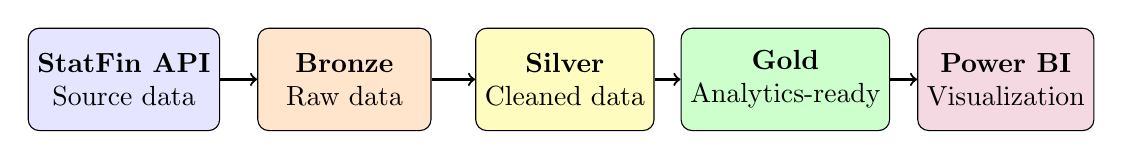
\begin{tikzpicture} 
% StatFin 
\node[ draw, rounded corners, fill=blue!10, minimum width=2.2cm, minimum height=1.3cm, align=center ] (statfin) at (0,0) {\textbf{StatFin API}\\Source data}; 
% Bronze 
\node[ draw, rounded corners, fill=orange!20, minimum width=2.2cm, minimum height=1.3cm, align=center ] (bronze) at (2.8,0) {\textbf{Bronze}\\Raw data}; 
% Silver 
\node[ draw, rounded corners, fill=yellow!25, minimum width=2.2cm, minimum height=1.3cm, align=center ] (silver) at (5.6,0) {\textbf{Silver}\\Cleaned data}; 
% Gold 
\node[ draw, rounded corners, fill=green!20, minimum width=2.2cm, minimum height=1.3cm, align=center ] (gold) at (8.4,0) {\textbf{Gold}\\Analytics-ready}; 
% Power BI 
\node[ draw, rounded corners, fill=purple!15, minimum width=2.2cm, minimum height=1.3cm, align=center ] (powerbi) at (11.2,0) {\textbf{Power BI}\\Visualization}; 
% Arrows 
\draw[->, thick] (statfin) -- (bronze); \draw[->, thick] (bronze) -- (silver); \draw[->, thick] (silver) -- (gold); \draw[->, thick] (gold) -- (powerbi); \end{tikzpicture} \vspace{0.8cm} \begin{itemize} \item \textbf{Databricks} handles data extraction, transformation and storage. \item \textbf{Delta tables} provide structured and queryable storage between processing layers. \item \textbf{Power BI} connects to the Gold layer for analysis and visualization. \item \textbf{GitHub} contains the project code, documentation and report screenshots. \end{itemize} \end{frame}

% ================================================= 
% Slide 5: Data extraction 
% ================================================= 
\begin{frame}[fragile]{Data Extraction from the StatFin API} \small The StatFin PXWeb API was queried with Python. The request selected the years 2008--2024 and returned the data in JSON-stat2 format. \vspace{0.2cm} \begin{lstlisting}[ 
style=pythonstyle, basicstyle=\ttfamily\tiny 
] 
years = [str(year) for year in range(2008, 2025)] 

payload = { 
    "query": [{ 
        "code": "Vuosi", 
        "selection": { 
            "filter": "item", 
            "values": years 
        } 
    }], 
    "response": {"format": "json-stat2"} 
} 

response = requests.post(api_url, json=payload) 
response.raise_for_status() 
\end{lstlisting} 
\vspace{0.15cm} 
\begin{alertblock}{Key processing step} The multidimensional JSON-stat2 response was transformed into a tabular structure suitable for Spark processing. \end{alertblock} 
\end{frame}

% ================================================= 
% Slide 6: Medallion architecture 
% ================================================= 
\begin{frame}{Bronze, Silver and Gold Layers} \small \begin{columns}[T,onlytextwidth] \begin{column}{0.31\textwidth} \begin{block}{Bronze} \textbf{Purpose:} Preserve source data \vspace{0.2cm} \begin{itemize} \setlength{\itemsep}{0.15cm} \item Raw API response \item Original values retained \item Supports traceability \end{itemize} \end{block} \end{column} \begin{column}{0.31\textwidth} \begin{block}{Silver} \textbf{Purpose:} Clean and standardise \vspace{0.2cm} \begin{itemize} \setlength{\itemsep}{0.15cm} \item English column names \item Correct data types \item Cleaned categories \end{itemize} \end{block} \end{column} \begin{column}{0.31\textwidth} \begin{block}{Gold} \textbf{Purpose:} Prepare for analysis \vspace{0.2cm} \begin{itemize} \setlength{\itemsep}{0.15cm} \item Industry hierarchy \item Injury categories \item Reporting-ready Delta table \end{itemize} \end{block} \end{column} \end{columns} \vspace{0.45cm} \begin{alertblock}{Design principle} Each layer has one clear responsibility: \textbf{Bronze preserves}, \textbf{Silver cleans}, and \textbf{Gold prepares the data for Power BI}. \end{alertblock} \end{frame}

% ================================================= 
% Slide 7: Transformations 
% ================================================= 
\begin{frame}{Important Data Transformations} \small \begin{block}{Transformation challenge} The original industry variable combined industry codes, hierarchy levels, descriptions and special categories in a single field. \end{block} \vspace{0.0cm} \begin{columns}[T,onlytextwidth] \begin{column}{0.31\textwidth} \begin{block}{Original field} \begin{itemize} \setlength{\itemsep}{0.12cm} \item Industry code \item Industry name \item Mixed hierarchy \item Special values \end{itemize} \end{block} \end{column} \begin{column}{0.31\textwidth} \begin{block}{Transformation} \begin{itemize} \setlength{\itemsep}{0.12cm} \item Extract code \item Identify level \item Separate labels \item Handle exceptions \end{itemize} \end{block} \end{column} \begin{column}{0.31\textwidth} \begin{block}{Gold fields} \begin{itemize} \setlength{\itemsep}{0.12cm} \item \texttt{industry\_code\_main} \item \texttt{industry\_code\_sub} \item \texttt{industry\_main} \item \texttt{industry\_sub} \end{itemize} \end{block} \end{column} \end{columns} \vspace{0.0cm} \begin{alertblock}{Special cases retained} Special categories, the local government sector and unknown values were handled explicitly instead of being removed. \end{alertblock} \end{frame}

% =================================================
% Slide 8: Power BI
% =================================================
\begin{frame}{Power BI Report}

\begin{columns}[T]

\column{0.46\textwidth}

\textbf{Report pages}

\begin{itemize}
    \item Information page
    \item Overview
    \item Industry analysis
    \item Demographic analysis
    \item Injury severity analysis
\end{itemize}

\textbf{Interactive functionality}

\begin{itemize}
    \item Year and industry filters
    \item KPI cards
    \item Drill-down through industry levels
    \item Custom category sorting
    \item Report-page tooltips
\end{itemize}

\column{0.50\textwidth}

\begin{figure} \centering \includegraphics[ width=\textwidth, height=5.2cm, keepaspectratio ]{overview.png} \caption{Power BI overview page} \end{figure}

\end{columns}

\end{frame}

% =================================================
% Slide 9: Main findings
% =================================================
\begin{frame}{Main Findings}

\begin{block}{1. Long-term development}
The annual number of occupational accidents
\alert{decreased} between 2008 and 2024.

The number decreased from approximately \alert{153 000} to \alert{119 000}, representing an overall decrease of approximately \alert{22.1\%}.
\end{block}

\begin{block}{2. Largest annual change}
The most notable year-on-year change occurred between
\alert{2019} and \alert{2020}, when accident volume
\alert{decreased} by approximately \alert{18\%}.
\end{block}

\begin{block}{3. Recent development}
During the most recent five years, occupational accident volumes have remained \alert{relatively stable}.
\end{block}


\end{frame}

% =================================================
% Slide 10: Industry findings
% =================================================
\begin{frame}{Findings by Industry}

\begin{columns}[T]

\column{0.48\textwidth}

\begin{block}{Highest accident volume}
The highest number of recorded occupational accidents was found in the
\alert{Local government -sector}.

In \alert{2024}, this industry represented approximately
\alert{24.4\%} of the accidents analyzed.
\end{block}

\begin{block}{Change over time}
The most substantial increase was observed in
\alert{Human health and social work activities (+83.9\%)}, while \alert{Manufacturing} showed the clearest decline \alert{(-59.5\%)}.
\end{block}

\column{0.48\textwidth}

\begin{figure} \centering \includegraphics[ width=\textwidth, height=5.2cm, keepaspectratio ]{top 10 industries.png} \caption{Top 10 industries by accidents} \end{figure}

\end{columns}

\end{frame}

% ================================================= 
% Slide 11: Demographic findings 
% ================================================= 
\begin{frame}{Demographic Findings} \small \begin{columns}[T,onlytextwidth] \begin{column}{0.47\textwidth} \begin{block}{Gender} \begin{itemize} \setlength{\itemsep}{0.08cm} \item \alert{Men} accounted for more recorded accidents. \item The largest gender difference occurred in \alert{construction}. \end{itemize} \end{block} \end{column} \begin{column}{0.50\textwidth} \begin{block}{Age group} \begin{itemize} \setlength{\itemsep}{0.08cm} \item The highest volumes occurred among \alert{25--34} and \alert{45--54-year-olds}. \item The lowest volume occurred among \alert{15--24-year-olds}. \end{itemize} \end{block} \end{column} \end{columns} \vspace{0.15cm} \begin{block}{Industry differences by age} \begin{itemize} \setlength{\itemsep}{0.08cm} \item Older profile: \alert{agriculture, forestry and fishing} and the \alert{local government sector}. \item Younger profile: \alert{accommodation and food services} and \alert{administrative and support services}. \end{itemize} \end{block} \vspace{0.1cm} \centering \footnotesize \textit{These figures describe accident volumes, not individual risk.} \end{frame}

% ================================================= 
% Slide 12: Injury severity 
% ================================================= 
\begin{frame}{Injury Severity Findings} \small \begin{block}{1. Short-duration injuries dominate} In 2024, \alert{66\%} of occupational accidents resulted in only \alert{0--3 days} of absence. \end{block} \vspace{0.15cm} \begin{block}{2. Fatal accidents} Fatal accidents were recorded most frequently in \alert{transportation and storage} and \alert{construction}. \end{block} \vspace{0.15cm} \begin{block}{3. Severity varies with age} Short-duration injuries were the most common across all age groups, but \alert{longer-duration injuries represented a larger share in older age groups}. \end{block} \vspace{0.15cm} \centering \footnotesize \textit{The findings describe the distribution of recorded accidents.} \end{frame}

% =================================================
% Slide 13: Limitations
% =================================================
\begin{frame}{Limitations}

\begin{enumerate}
    \item \textbf{Counts are not accident rates}

    The dataset describes the number of accidents but does not directly
    adjust for the number of employees or hours worked.

    \item \textbf{Workforce composition affects comparisons}

    Differences by gender, age or industry may partly reflect the size
    and structure of the underlying workforce.

    \item \textbf{Classification changes}

    Industry classifications or reporting practices may have changed
    during the 2008--2024 period.

    \item \textbf{Aggregated data}

    The data does not support analysis of individual accident circumstances,
    causes or detailed risk factors.

\end{enumerate}

\end{frame}

% =================================================
% Slide 14: Skills demonstrated
% =================================================
\begin{frame}{Skills Demonstrated}

\begin{columns}[T]

\column{0.31\textwidth}
\begin{block}{Data Engineering}
\begin{itemize}
    \item REST API requests
    \item JSON-stat processing
    \item PySpark transformations
    \item Delta tables
    \item Medallion architecture
\end{itemize}
\end{block}

\column{0.31\textwidth}
\begin{block}{Data Analytics}
\begin{itemize}
    \item Data validation
    \item Trend analysis
    \item Category design
    \item DAX measures
    \item Contextual interpretation
\end{itemize}
\end{block}

\column{0.31\textwidth}
\begin{block}{Communication}
\begin{itemize}
    \item Power BI reporting
    \item Interactive tooltips
    \item GitHub documentation
    \item Visual storytelling
    \item Limitations and conclusions
\end{itemize}
\end{block}

\end{columns}

\end{frame}

% =================================================
% Slide 15: Conclusion
% =================================================
\begin{frame}{Conclusions and Next Steps}

\begin{block}{Conclusion}
The project demonstrates how public statistical data can be transformed
into a reproducible analytics solution. It connects data acquisition,
engineering, modelling, visualization and communication in a single workflow.
\end{block}

\vspace{0.3cm}

\textbf{Potential next steps}

\begin{itemize}
    \item Add employment data to calculate accident rates
    \item Add hours worked as an exposure measure
    \item Automate annual data refreshes
    \item Add data-quality tests to the Databricks pipeline
    \item Compare occupational accidents with economic or labor-market indicators
\end{itemize}

\end{frame}

% =================================================
% Slide 16: Questions
% =================================================
\begin{frame}
    \centering
    \Huge Questions?

    \vspace{0.8cm}

    \large
    Sonja Kurri

    \vspace{0.3cm}

    \normalsize
    GitHub: \alert{https://github.com/sonjacurry/occupational-accidents-demo}\\
    LinkedIn: \alert{www.linkedin.com/in/sonja-kurri}
\end{frame}

\end{document}